\documentclass{article}

% The amsmath and epsfig packages greatly simplify the process of adding
% equations and figures to the document, and thus their use is highly
% recommended.
% ------------
\usepackage{spconf,mathtools,epsfig}
\usepackage{url}
\usepackage{float}
\usepackage{subcaption}
\usepackage{cleveref}
\usepackage{listings}
\usepackage[style=ieee]{biblatex}
\usepackage{blindtext}

% image folder
\graphicspath{{./images/}}

% bib file
\bibliography{report}

% Title.
% ------
\title{SGN-16006,
  Auditory Scene Recognition
}



\name{Jonas Nikula, Vili Saura
%\thanks{Insert sponsor acknowledgments (where necessary) here.}
}
%
\address{240497, 240264\\
%University / Company\\
%Address\\
jonas.nikula@student.tut.fi, vili.saura@student.tut.fi}

% Hyphenation (hyphenate all names and non-english words here).
% -------------------------------------------------------------
\hyphenation{Tam-pe-re micro-soft}

\begin{document}

\maketitle
\sloppy

% include sections here
\section{Introduction}
We've used Python 3.6 in this assignment.


\section{Background theory}
In telephone networks the dialed number is transmitted  with DTMF signals. Every number is  a result of two frequencies, as seen in  figure~\ref{fig:DTMF}. We used two algorithms that detected the vertical frequencies and calculated the amount of this frequency in the signal. This amount is then compared to a threshold, and if it is greater than the threshold, a corresponding LED will light.

\begin{figure}[H]
  \centering
  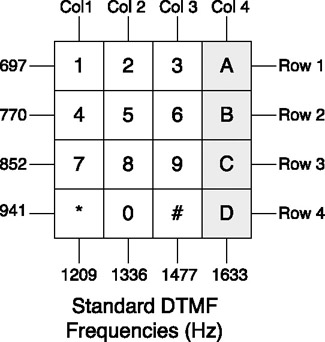
\includegraphics[width=0.8\linewidth]{DTMF}
  \caption{DTMF frequencies ~\cite{DTMF}}
\label{fig:DTMF}
\end{figure}

 Two different methods were used in this assignment, Correlation detection and Goertzel -algorithm. In the first method we calculated the correlation between the input data and and the signals ~\ref{eq:cos} and ~\ref{eq:sin}.

\begin{equation}
  \label{eq:cos}
  c_{697}(n) = \cos(2 \pi \times 697 \times n/F_{n})
\end{equation}

\begin{equation}
  \label{eq:sin}
  s_{697}(n) = \sin(2 \pi \times 697 \times n/F_{n})
\end{equation}

The correlations are defined by equations ~\ref{eq:corCos} and ~\ref{eq:corSin}.

\begin{equation}
  \label{eq:corCos}
  c_{\cos}(697) =\sum_{n=0}^{N-1} c_{697}(n)  \times x(n)
\end{equation}

\begin{equation}
  \label{eq:corSin}
  c_{\sin}(697) =\sum_{n=0}^{N-1} s_{697}(n)  \times x(n)
\end{equation}

Next we estimated the signal power using equation ~\ref{eq:var}.

\begin{equation}
  \label{eq:var}
  var =\sum_{n=0}^{N-1}x(n)^2
\end{equation}

Finally, we tested the presence of the frequency using equation ~\ref{eq:pres} In this case, we tested the presence of the 697Hz component. By replacing the 697 value in the equations, we can test the presence of the other components.

\begin{equation}
  \label{eq:pres}
 w_{697} =\frac {c^2_{cos}(697) + c^2_{sin}(697)}{var}
\end{equation}

The Goertzel-algorithm uses an unstable IIR filter that amplifies the selected frequencies. Detecting the frequency f with sampling frequency $F_{s}$ can be done using Goetzel filter ~\ref{eq:gFilter}.

\begin{equation}
  \label{eq:gFilter}
  y(n) =x(n) + 2\cos(2 \pi f/F_{s})y(n-1) - y(n-2)
\end{equation}

\begin{equation}
  \label{eq:gFilter}
  y(n) =x(n) + 2\cos(2 \pi f/F_{s})y(n-1) - y(n-2)
\end{equation}

However, we cannot use this equation as a direct indication on which LED should light. Instead, we can use equation ~\ref{eq:gFinal}.

\begin{equation}
  \label{eq:gFinal}
  |Y(e^{(i \omega)}|^2 = y^2(N-1) + y^2(N-1) - 2 \cos(2 \pi f/F_{s})y(N-2)y(N-1)
\end{equation}

The Goertzel algorithm itself consists of three steps. We loop through all the steps, increasing the value of n with every step. Step 1. we initialize n , y(n-1) and y(n-2) as 0. Then in step 2, if n < N we calculate y(n) using ~\ref{eq:gFilter}, increment n = n+1 and return to step 2.In step 3, if n  is equal to N,  we calculate ~\ref{eq:gFinal}. and divide it with variance, using equation ~\ref{eq:var}.
This value is compared to the thresholdn and if it is greater than the threshold, LED is turned on, otherwise it's turned off. Again, we increment n=n+1 and return to step 1.
\section{Methods}

\subsection{Nearest neighbor interpolation}
In nearest neighbor interpolation, we process the raw Bayer data in squares of
4 pixels, which contain 1 red, 1 blue and 2 green pixels. For the blue
channel, all 4 pixels are set to the color value of the 1 blue pixel. The same
is done for the red channel. For the green channel, the pixels without a green
color value get their value from the green pixel horizontally next to them.

The main benefits of NN-interpolation are its speed and simplicity.

\subsection{Bilinear interpolation}

In bilinear interpolation the color value of the pixels is calculated from the
color value of neighboring pixels with same color i.e sum the values of
neighboring pixels and divide it by the amount of neighboring pixels. However,
the pixels at the edges of the picture don't always have neighboring pixels
with color value or don't have enough of them. To correct this we can just
ignore the border pixels, resulting in smaller image, or as we did in the
assignment and pad the color arrays with zeros. The color values of the layers
are in different pixels, so every layer needs an unique function to calculate
the value of an unknown pixel.  Green has the most known color values, and
every unknown pixel borders four known pixels, so one function can calculate
all values of the green layer.

Only every other row of red and green layers has colorvalues, which has to be
taken into account when designing these functions. The rows which have no
colorvalues compute the value differently, depending on how many known values
border the pixel, and use either four or two values.

Colorvalues of the pixels are calculated from the padded color array and added
to the unpadded one. After all values of all colorarrays are calculated, the
arrays are combined into RGB image.

\subsection{Patterned pixel grouping interpolation}
The Patterned Pixel Grouping, or PPG interpolation is a significantly more
advanced method of interpolation. We implemented the method using the
description found here\cite{chuan-kai_lin}.

This method basically tries to take into account the color gradients found in
the data. It also takes advantage of the greater amount of green data and uses
it to assess the brightness gradients of the image, which is a feature that the
human visual system perceives more accurately than changes in color.

First the method calculates a value for all the missing green pixels. It
calculates the values by first assessing 4 gradients, in the cardinal
directions, using two neighboring green pixels and the red/blue pixel in place
of the missing green pixel and the red/blue pixel in the cardinal direction.

The pixels used in the calculation of the smallest gradient are then used to
calculate the actual green color value for the pixel.

\section{Results}

The~\cref{fig:nnInterpolation,fig:blInterpolation,fig:ppgInterpolation}
contain two images that are obtained by processing the raw Bayer data with our
implemented interpolation methods.

\begin{figure}[H]
\centering
\begin{subfigure}{.25\textwidth}
  \centering
  
\includegraphics[width=.9\linewidth]{nnCrop2}
  \caption{image 2}
\label{fig:nnCrop2}
\end{subfigure}%
\begin{subfigure}{.25\textwidth}
  \centering
  
\includegraphics[width=.9\linewidth]{nnCrop5}
  \caption{image 5}
\label{fig:nnCrop5}
\end{subfigure}
\caption{A zoomed in area of two NN-interpolation processed images}
\label{fig:nnInterpolation}
\end{figure}


\begin{figure}[H]
\centering
\begin{subfigure}{.25\textwidth}
  \centering
  
\includegraphics[width=.9\linewidth]{blCrop2}
  \caption{image 2}
\label{fig:blCrop2}
\end{subfigure}%
\begin{subfigure}{.25\textwidth}
  \centering
  
\includegraphics[width=.9\linewidth]{blCrop5}
  \caption{image 5}
\label{fig:blCrop5}
\end{subfigure}
\caption{A zoomed in area of two bilinear interpolation processed images}
\label{fig:blInterpolation}
\end{figure}


\begin{figure}[H]
\centering
\begin{subfigure}{.25\textwidth}
  \centering
  
\includegraphics[width=.9\linewidth]{ppgCrop2}
  \caption{image 2}
\label{fig:ppgCrop2}
\end{subfigure}%
\begin{subfigure}{.25\textwidth}
  \centering
  
\includegraphics[width=.9\linewidth]{ppgCrop5}
  \caption{image 5}
\label{fig:ppgCrop5}
\end{subfigure}
\caption{A zoomed in area of two patterned pixel grouping interpolation processed images}
\label{fig:ppgInterpolation}
\end{figure}


The table~\ref{tab:results} contains the Mean Squared Error, Mean Absolute
Error and time it took to run the interpolation function. The error rates were
obtained by processing the raw data with our implemented functions, and
comparing that result to a TIFF encoded file of the same data. The computation
times were obtained using Matlab's tic-toc timetaking function. They'll
depend on the computer used, but what can be objectively compared are their
relative durations.
\begin{table}[H]
  \centering
  \caption{Results from the different methods}
\label{tab:results}
  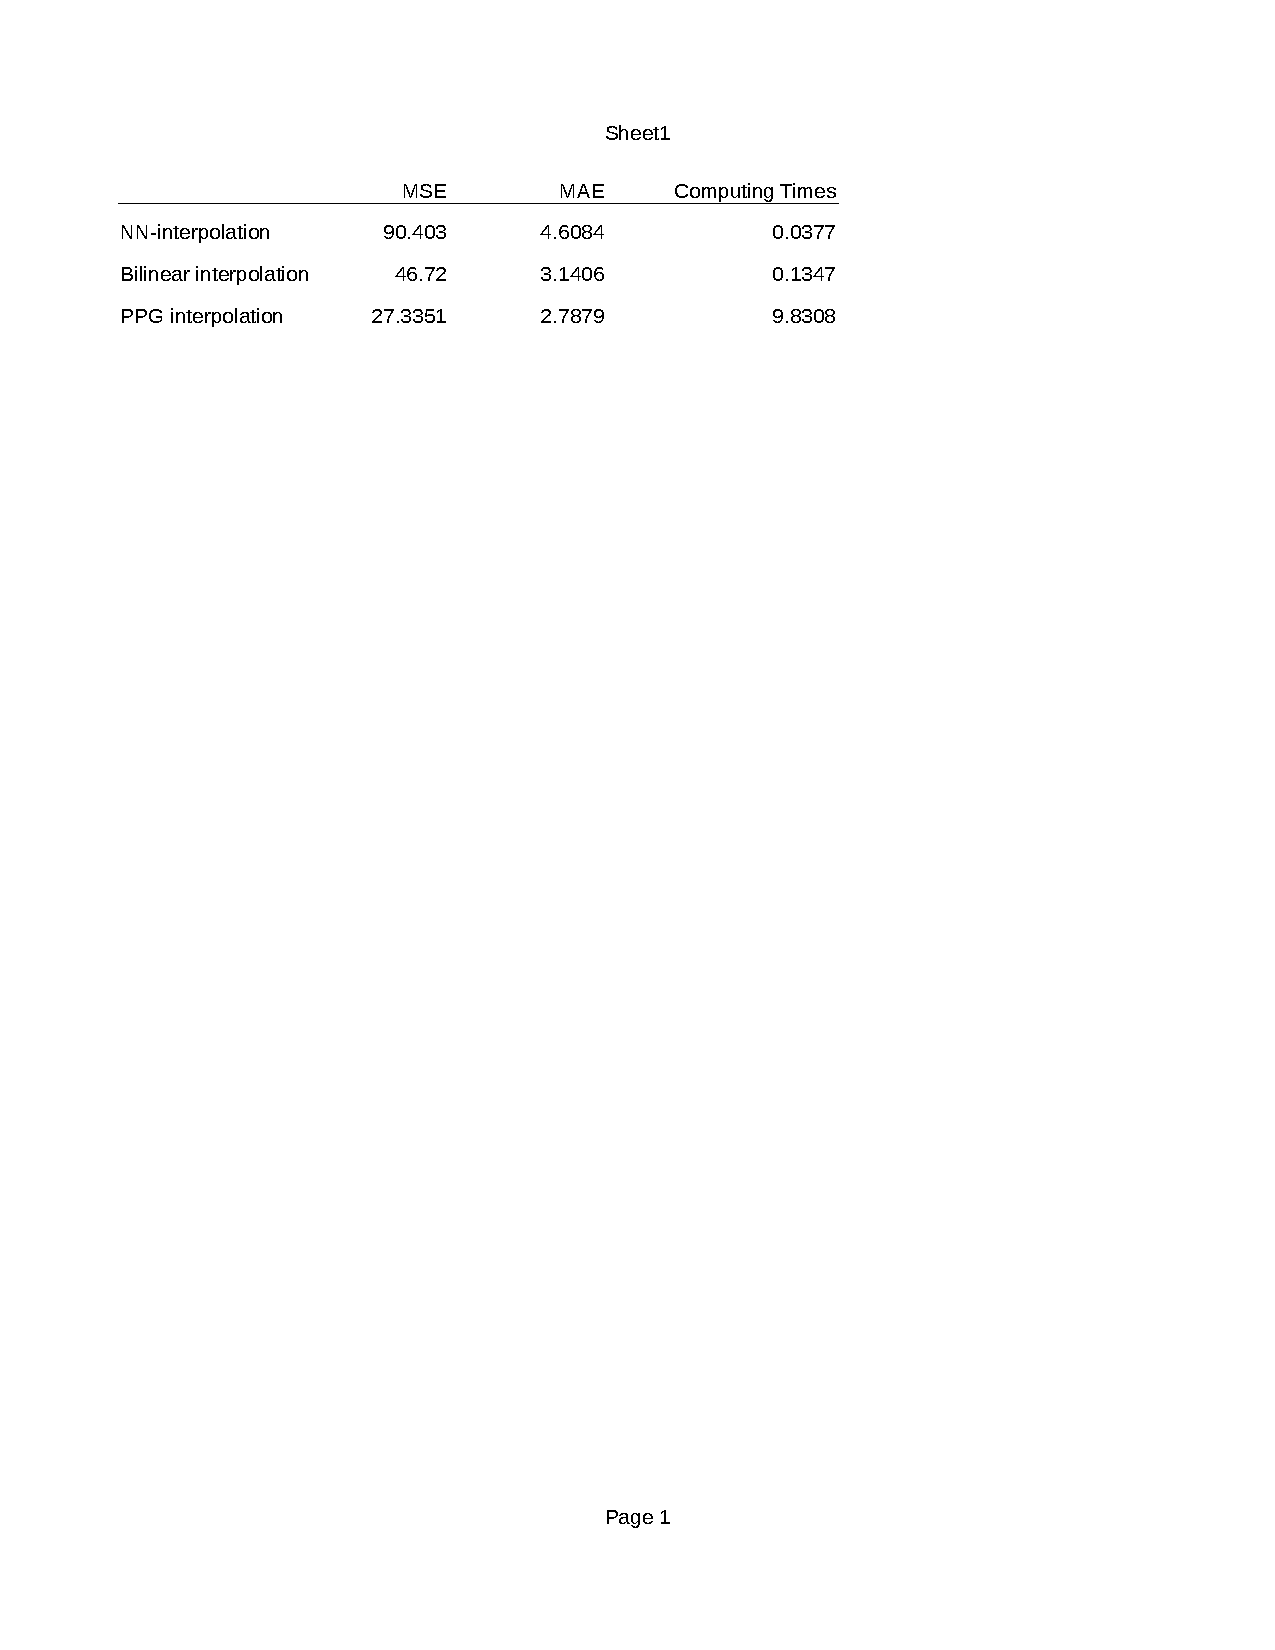
\includegraphics[width=1\linewidth]{results_table}
\end{table}



\section{Conclusions}
With correct parameters the threshold can be found experimentally. At first, we tested correlation detection with sampling frequency of 44100Hz and period of 10µs. These parameters worked  with the first part of the Matlab code, resulting in threshold of 90. However, this threshold wouldn't work with the other Matlab tests. Then we changed the values to 3000HZ and 333µs and all test worked with threshold of 8. Goertzel-algorithm passed the tests with same values, but we had to start indexing n from 1.

\small

\printbibliography{}

% ---------------------------------------------------------------------------
\vfill\pagebreak

\end{document}
